\documentclass[11pt,fleqn]{article}
%\usepackage{CJK}
\usepackage{latexsym}
\usepackage{color}
\usepackage{graphicx, float}\usepackage{graphicx}
%\usepackage{algorithmicx}
\usepackage{algorithm}
\usepackage{algpseudocode}
%\usepackage[colorlinks]{hyperref}
\setlength{\oddsidemargin}{-0.0in}
\setlength{\evensidemargin}{-0.0in} \setlength{\textwidth}{6.0in}
\setlength{\textheight}{9.0in} \setlength{\topmargin}{-0.2in}

%\setlength{\leftmargin}{0.7in}
\usepackage{amssymb, graphicx, amsmath}  %  fancyheadings,
\usepackage{setspace}
\newcommand\qed{\qquad $\square$}
\newcommand{\nn}{\nonumber}

\def \[{\begin{equation}}
\def \]{\end{equation}}
\def\proof{{\bf Proof:\quad}}
\def \endzm {\quad $\Box$}
\def\dist{\hbox{dist}}


\newcommand{\R}{\mathbb{R}}
%\newtheorem{yinli}{����}[section]
\newcommand{\D}{\displaystyle}
\newcommand{\T}{\textstyle}
\newcommand{\SC}{\scriptstyle}
\newcommand{\FT}{\footnotesize}



%\newtheorem{theorem}{Theorem}[section]
%\renewcommand{\thetheorem}{\arabic{section}.\arabic{theorem}}
\newtheorem{definition}{Definition}
\renewcommand{\thedefinition}{\arabic{section}.\arabic{definition}}
\newtheorem{lemma}{Lemma}[section]
\renewcommand{\thelemma}{\arabic{section}.\arabic{lemma}}
\newtheorem{remark}{Remark}
\renewcommand{\theremark}{\arabic{section}.\arabic{remark}}
\newtheorem{proposition}{Proposition}[section]
\renewcommand{\theproposition}{\arabic{section}.\arabic{proposition}}
\newtheorem{corollary}{Corollary }[section]
\renewcommand{\thecorollary}{\arabic{section}.\arabic{corollary}}
\renewcommand{\theequation}{\arabic{section}.\arabic{equation}}
\renewcommand{\baselinestretch}{1.35}
\newtheorem{exam}{Example}[section]
\renewcommand{\theexam}{\arabic{section}.\arabic{exam}}
\newtheorem{theo}{Theorem}[section]
\renewcommand{\thetheo}{\arabic{section}.\arabic{theo}}
\begin{document}
%\begin{CJK*}{GBK}{song}

\begin{center}

{\LARGE \bf  Visual Recognition Assignment 2}\\


\vskip 25pt
 {Huihuang Zheng, huihuang@utexas.edu }\\
\vskip 5pt
{\small hz4674 Spring 2016 }

\end{center}

\begin{spacing}{1.5}
\section{Using Code}
To run my code, run the \textbf{main.m} with Matlab. First, it will call \textbf{matchComparsion} and shows figures of output matching lines between 3 images for SIFT for Thresholded nearest neighbors, Thresholded ratio test and Inliers. Second, it will call \textbf{detectObject} and outputs figures of object matching results. For every output image, you can see what it's for in the Matlab console. You need to input "dbcont" in Matlab console to see next output image. (as demo in the provided code)

\section{Algorithm Implementation}
\subsection{Threshold Nearest Matching}
See \textbf{thresMatch.m}. This function inputs two sets of descriptors. For each descriptor $d_1$ in first set, we calculate the Euclidean distances between all descriptors in second set. Then, we compute the mean distance. Every descriptor $d_i$ in first set is matched to $d_j$ in second set with smallest Euclidean distance. Then we eliminate those smallest distance is less than mean distance times threshold. In this assignment, I set threshold as 0.8.
\subsection{Threshold Ratio Matching}
See \textbf{ratioMatch.m}. Similar to \textbf{thresMatch.m}. This function inputs two sets of descriptors. For each descriptor $d_1$ in first set, we calculate the Euclidean distances between all descriptors in second set. But then we sort these distances. Every descriptor $d_i$ in first set is matched to $d_j$ in second set except whose nearest distance is greater than threshold times second nearest distance. In this assignment, I set threshold as 0.6;
\subsection{RANSAC Matching}
See \textbf{ransac.m}. This function takes location of points in image1 and that of corresponding points in image2 as input. The corresponding points are just nearest Euclidean matching. Then, using the RANSAC algorithm to get best affine function. We eliminate those points who are outliers of RANSAC. There are two problems here. How to get affine transformation from corresponding points and how to do RANSAC.
\subsubsection{Implement Affine}
Given
$$H =
\begin{pmatrix}
a & b & c \\
d & e & f \\
\end{pmatrix}
,
p_1 =
\begin{pmatrix}
x\\
y\\
1\\
\end{pmatrix}
,
p_2 =
\begin{pmatrix}
x'\\
y'\\
\end{pmatrix}
$$
We know $p_2 = Hp_1$. The $H$ is parameters for affine transformation. So:
$$x' = ax + by + c$$
$$y' = dx + ey + f$$
We have
$$
\begin{pmatrix}
x & y & 1 & 0 & 0 & 0\\
0 & 0 & 0 & x & y & 1\\
...
\end{pmatrix}
\begin{pmatrix}
a \\ b \\ c \\ d \\ e \\ f 
\end{pmatrix}
=
\begin{pmatrix}
x'\\
y'\\
...
\end{pmatrix}
$$
So when we have points $p_1$ and corresponding points $p2$ with location $x, y, x', y'$, we can get the affine transformation.

\subsubsection{Implement RANSAC}
From above, we know affine has 6 unknowns and each points pair can offer 2 equations. For every iteration, we choose 3 points randomly (at least we should have 3 points) to get an affine transformation. Then, we calculate the location $q'_i$ which is point $p_i$ in image1 affine transforming to image2. Then, for $p_i$'s corresponding point $q_i$, if distance between $q_i$ and $q'_i$ is less than threshold (I set threshold as $\frac{1}{10}$ of sum of height and width of image2 ), we said the $q_i$ is inlier. If number of inliers reaches a threshold (I set over 30\% points are inliers), I will calculate the average Euclidean distance of all inliers. Finally, I choose the affine transformation with smallest average Euclidean distance of all inliers.

\subsection{Object Matching}
See \textbf{detectObject.m}. For matching algorithm, I combine all three matching above: the matching points are under both constraints of nearest threshold and ratio threshold, then I use RANSAC to get affine transformation and draw rectangle in image2 to show matched object.

\section{Experiment}
I will show figures of result of my programs and extra examples in this section.
\subsection{Show SIFT matching lines between UT Tower}
In this section, I will show total 9 images which is the requirement of this assignment and analysis for result at last. 
\subsubsection{Thresholded Nearest Matching}

\begin{center}
  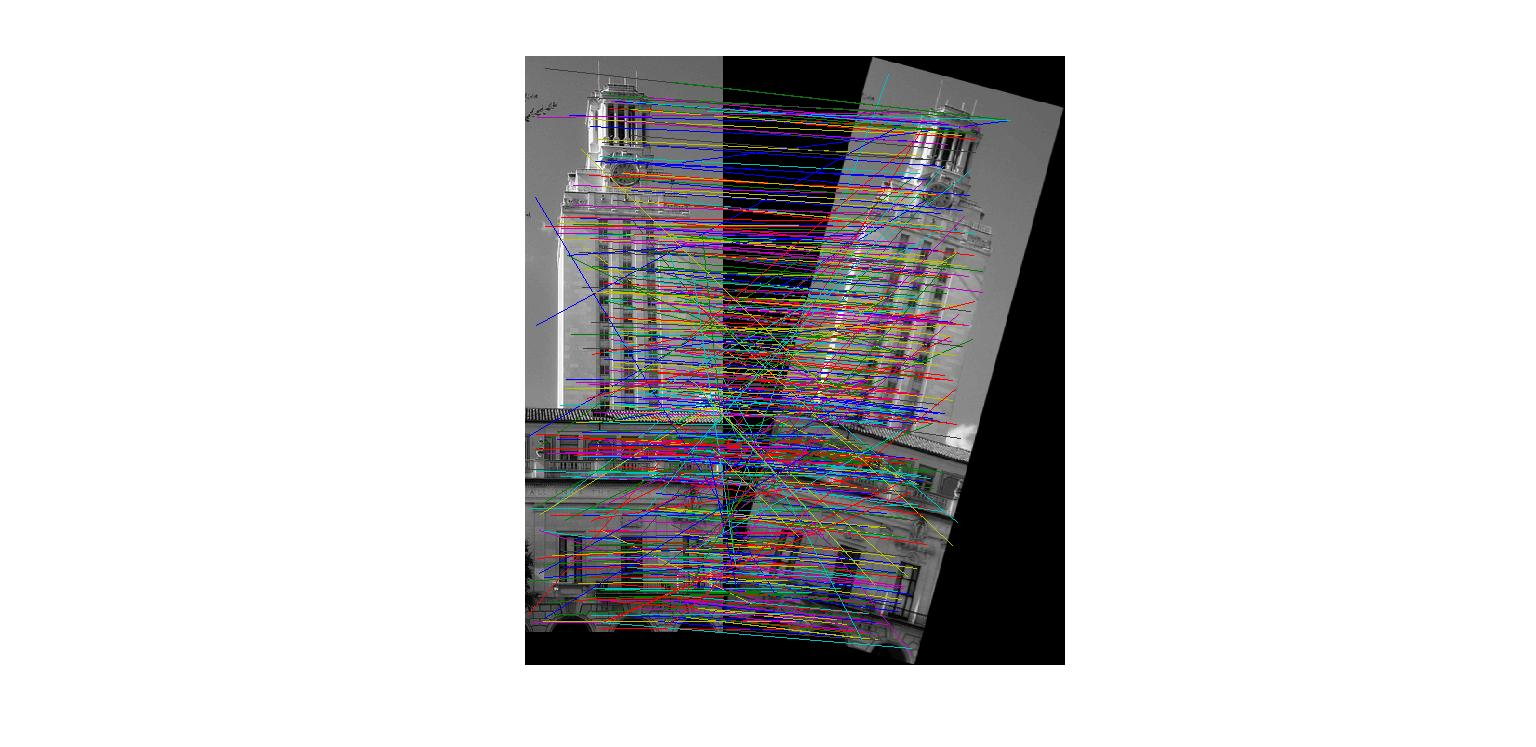
\includegraphics[width=0.8\linewidth]{thres_1.jpg}
  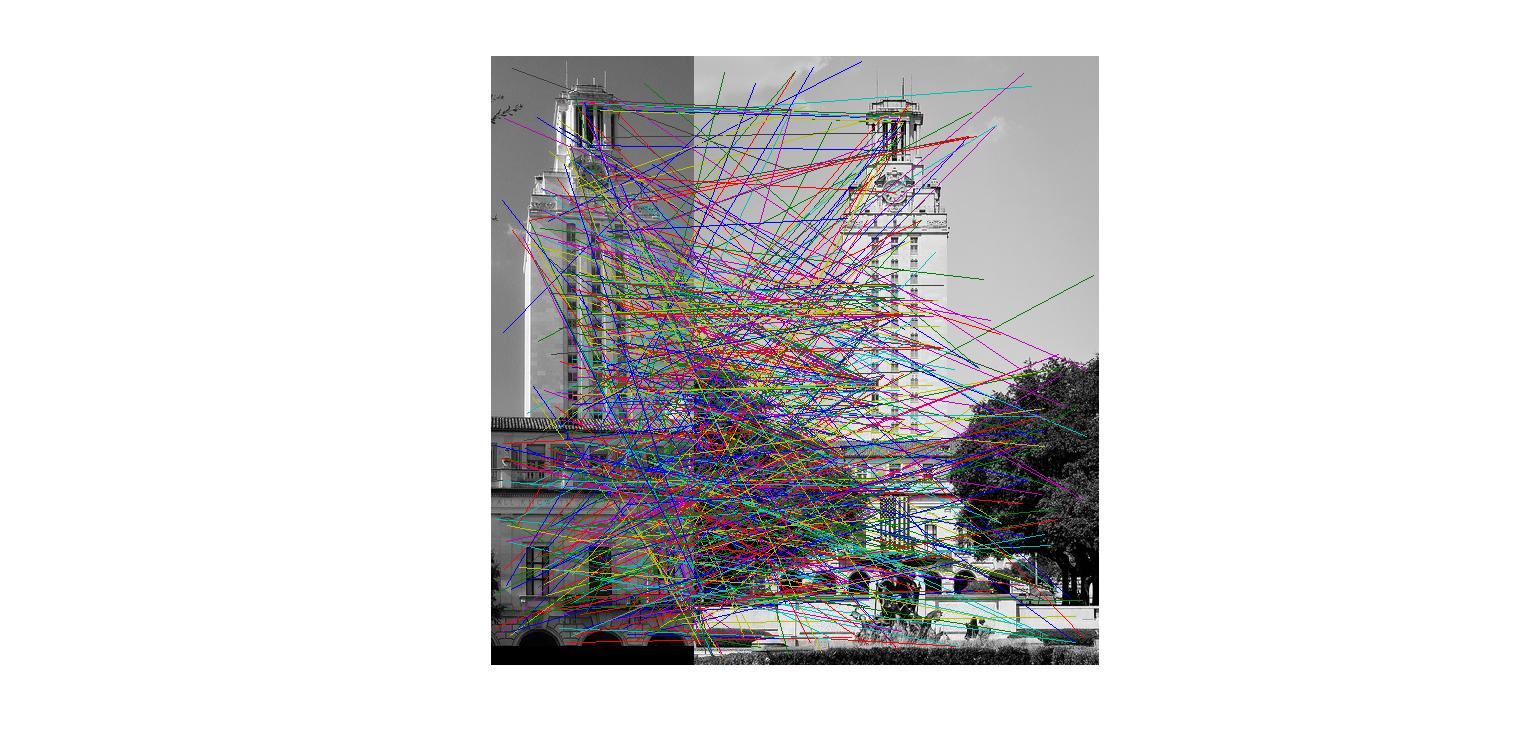
\includegraphics[width=0.8\linewidth]{thres_2.jpg}
  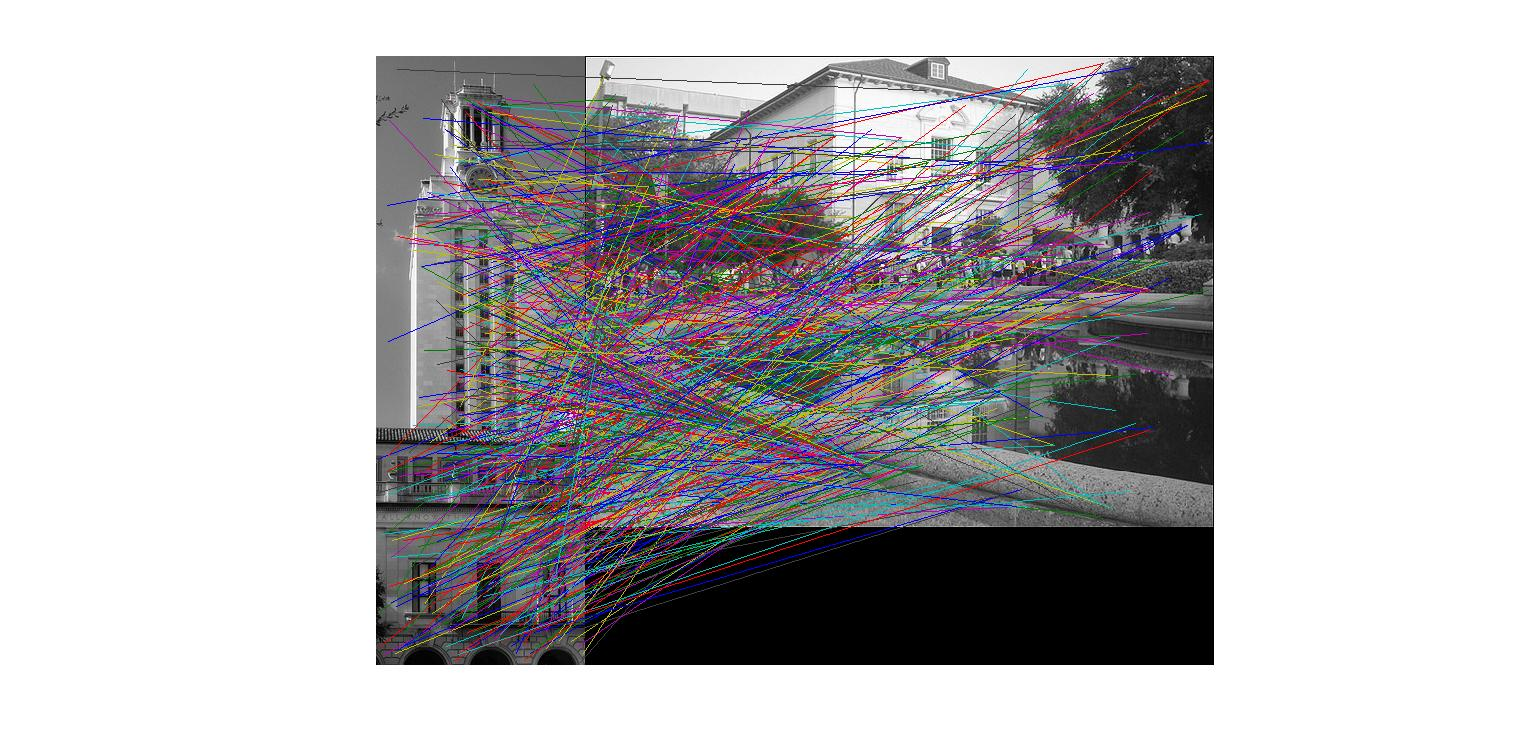
\includegraphics[width=0.8\linewidth]{thres_3.jpg}
\end{center}
\subsubsection{Thresholded Ratio Matching}
\begin{center}
  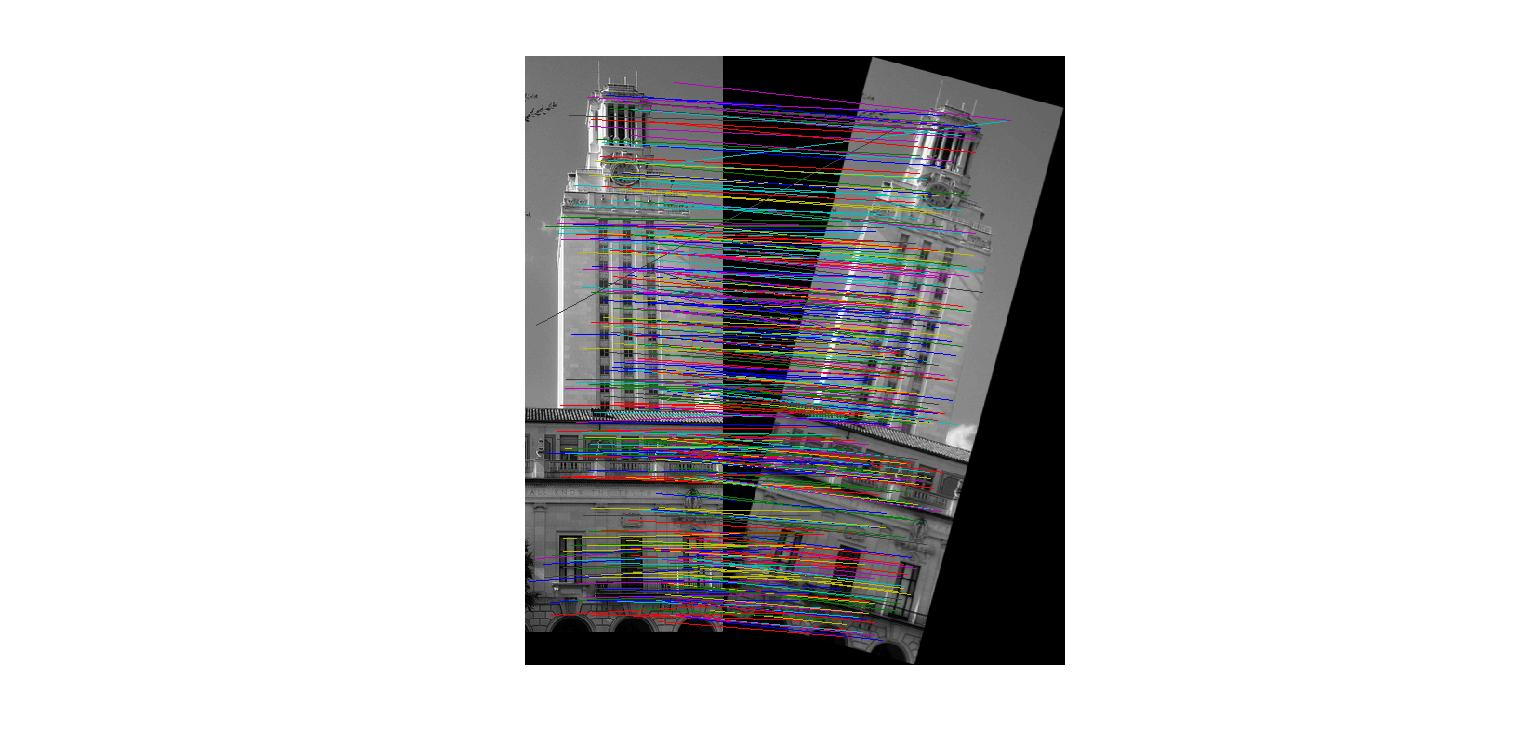
\includegraphics[width=0.8\linewidth]{ratio_1.jpg}
  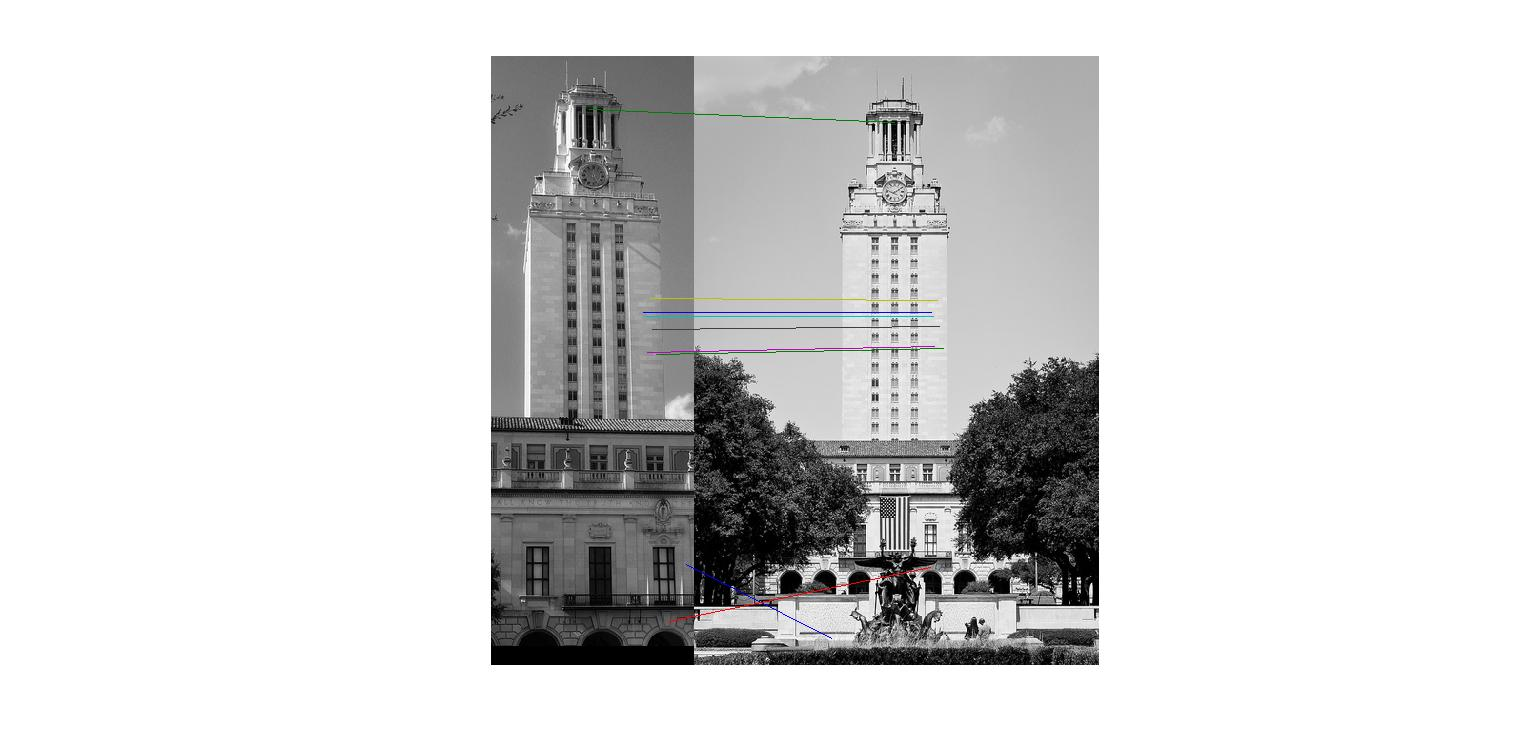
\includegraphics[width=0.8\linewidth]{ratio_2.jpg}
  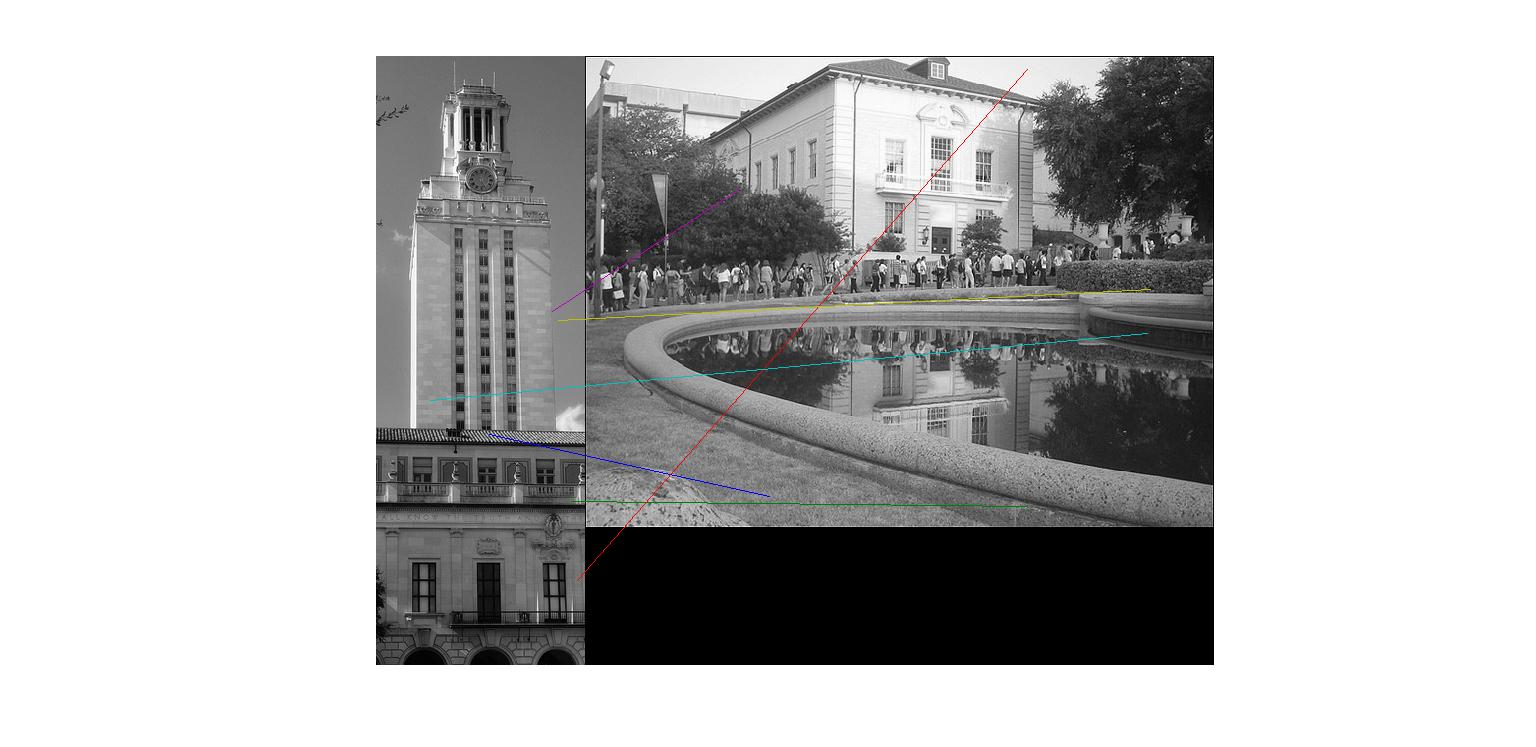
\includegraphics[width=0.8\linewidth]{ratio_3.jpg}
\end{center}
\subsubsection{Ransac Matching}
\begin{center}
  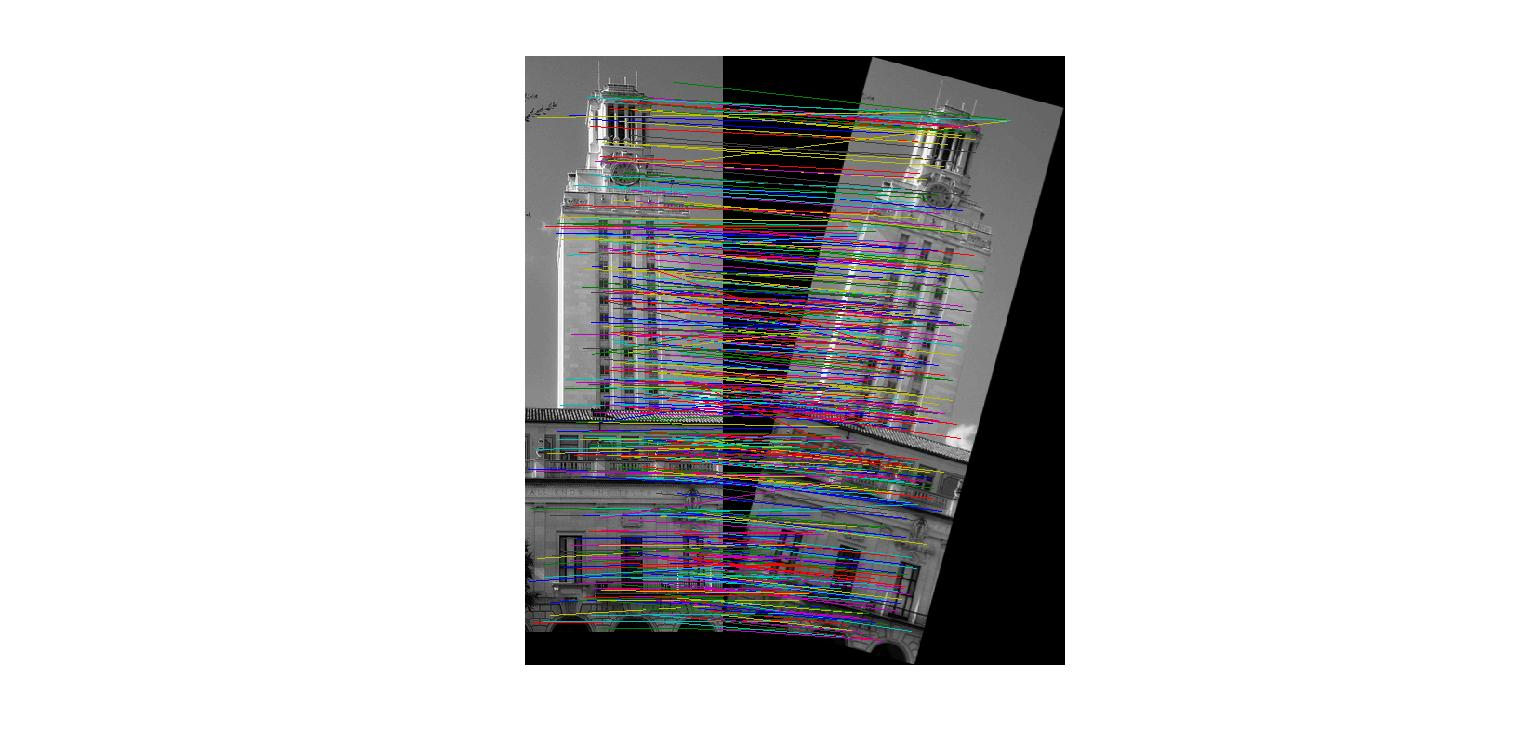
\includegraphics[width=0.8\linewidth]{inlier_1.jpg}
  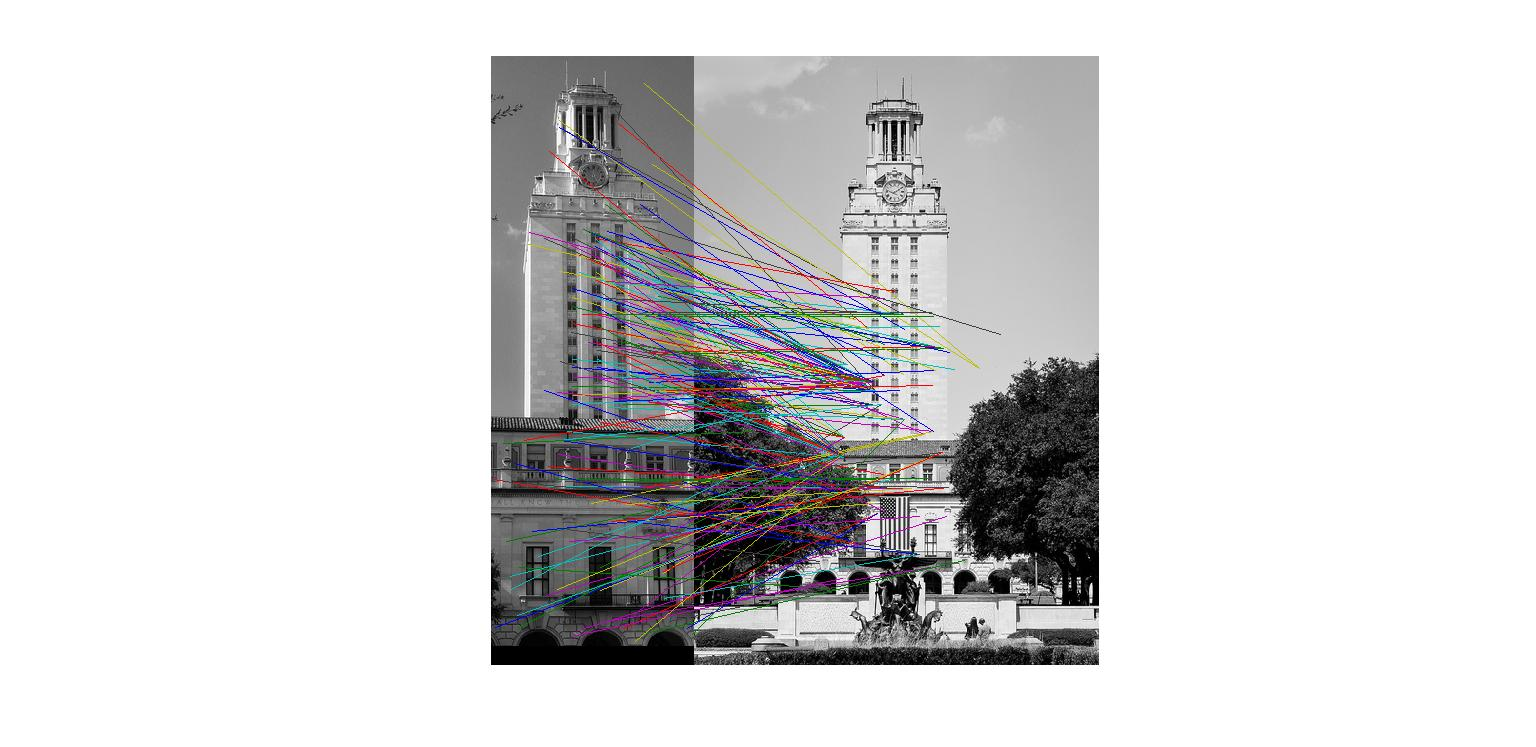
\includegraphics[width=0.8\linewidth]{inlier_2.jpg}
  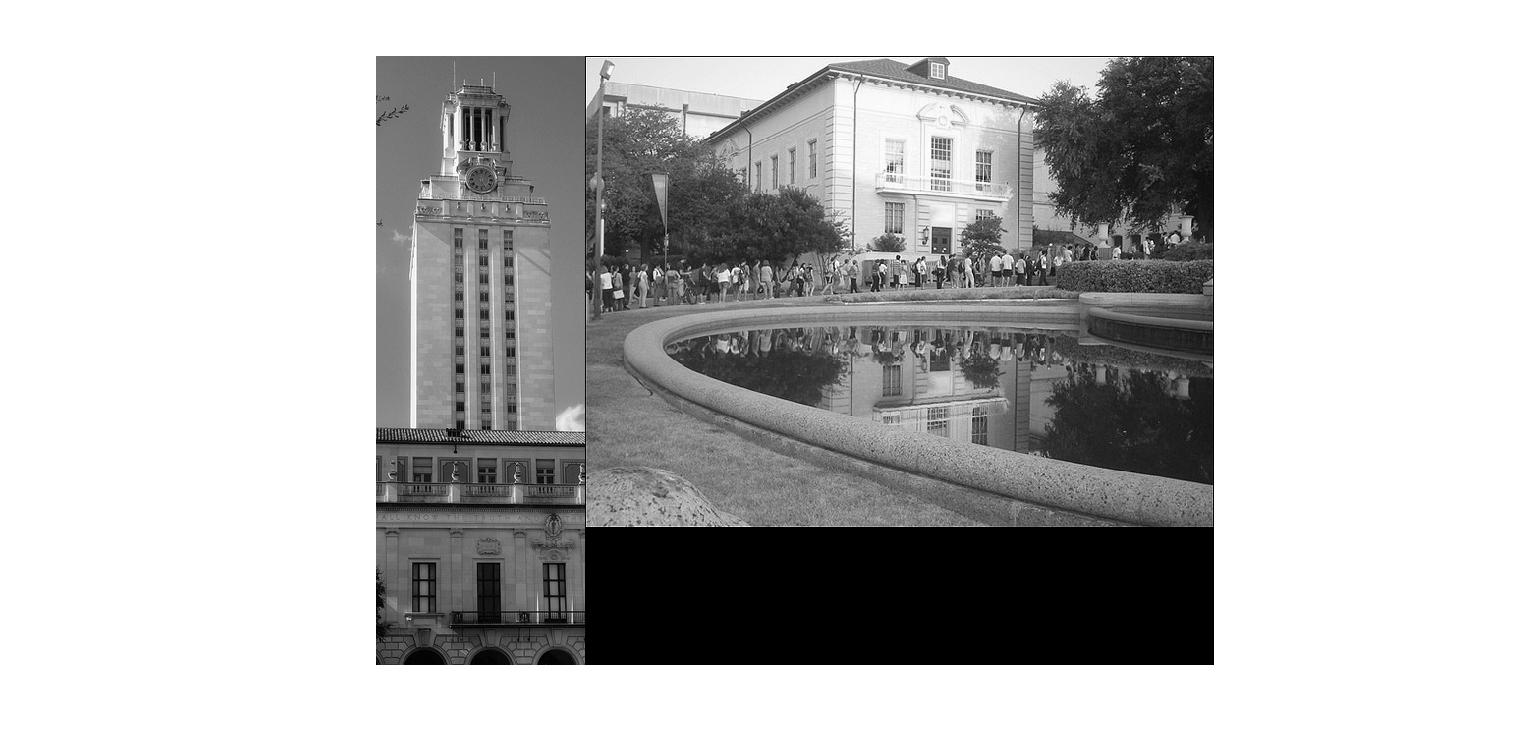
\includegraphics[width=0.8\linewidth]{inlier_3.jpg}
\end{center}

\subsubsection{Analyze Matching}
From those results, we can see that the thresholded nearest matching is the most unstable one, for first two images, a lot of unparallel matching, which suggest it's wrong matching.
In addition, it keeps a lot of matching in third image which doesn't have UT Tower at all. \\
Thresholed ratio matching is better. Fewer several unparallel matching in first two images, eliminate lots of matching pairs in image3. \\
RANSAC matching does best in image3 and image1, because RANSAC seeks location agreement, it eliminate all matchings in image3. In image1, it only keeps those almost parallel matching, because few unparallel matching was eliminated outliers. However, in image2, it isn't as better as Threshold ratio matching. It should be RANSAC can only find few location agreement and be mislead by raw nearest matching.

So the RANSAC and ratio matching have their different advantages. In object matching, I combine them: using ratio matching to get matching points and using RANSAC to check the spatial agreement.  
\subsection{Object Matching}

\subsubsection{UT TOWER}
In this section I show my matching results of UT tower image. You can see the program works well. Notice that in image3, we also have a rectangle. When I was hacking, I found there are only 3 pairs of matching survived after thresholded nearest and ratio checking. So these 3 points are major of RANSAC...
\begin{center}
  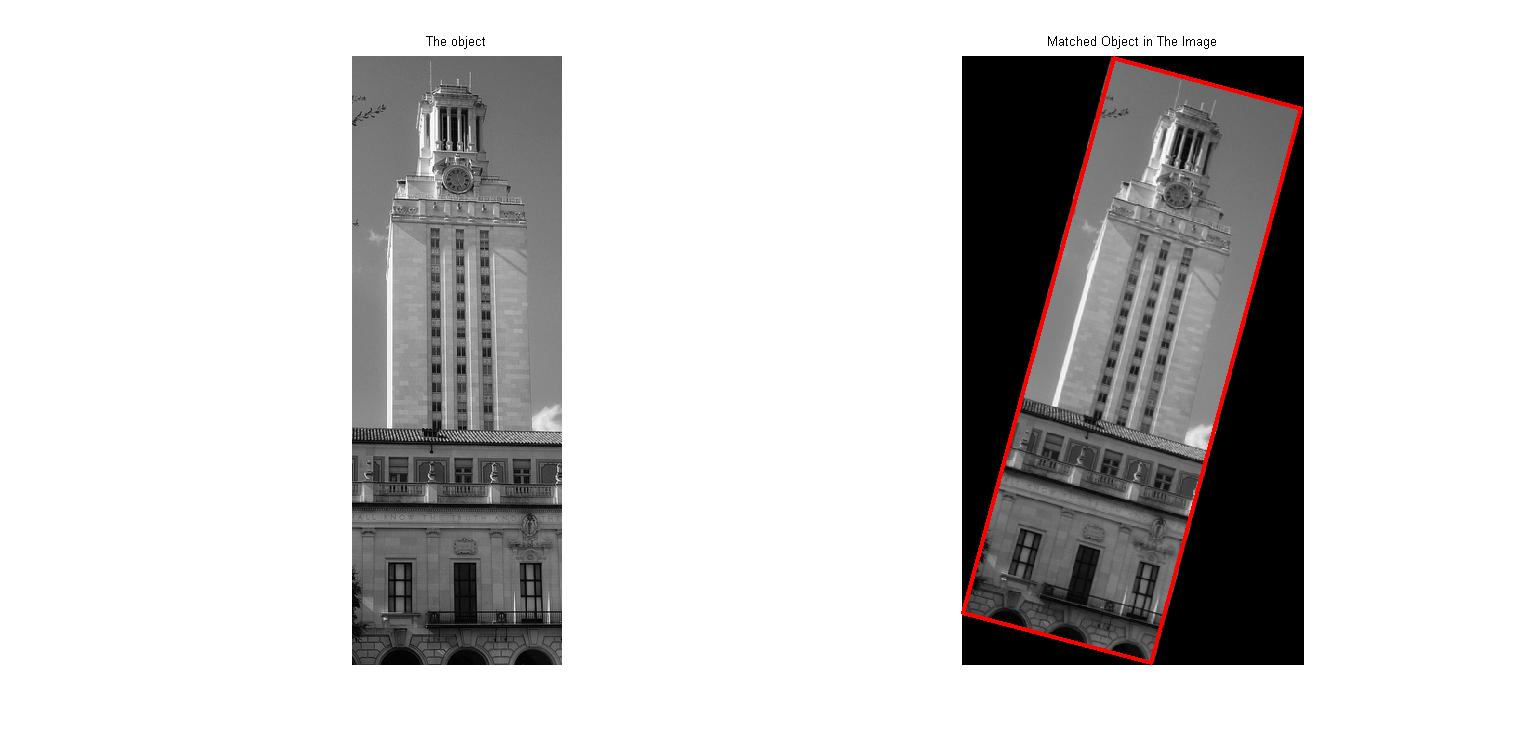
\includegraphics[width=\linewidth]{match_1.jpg}
  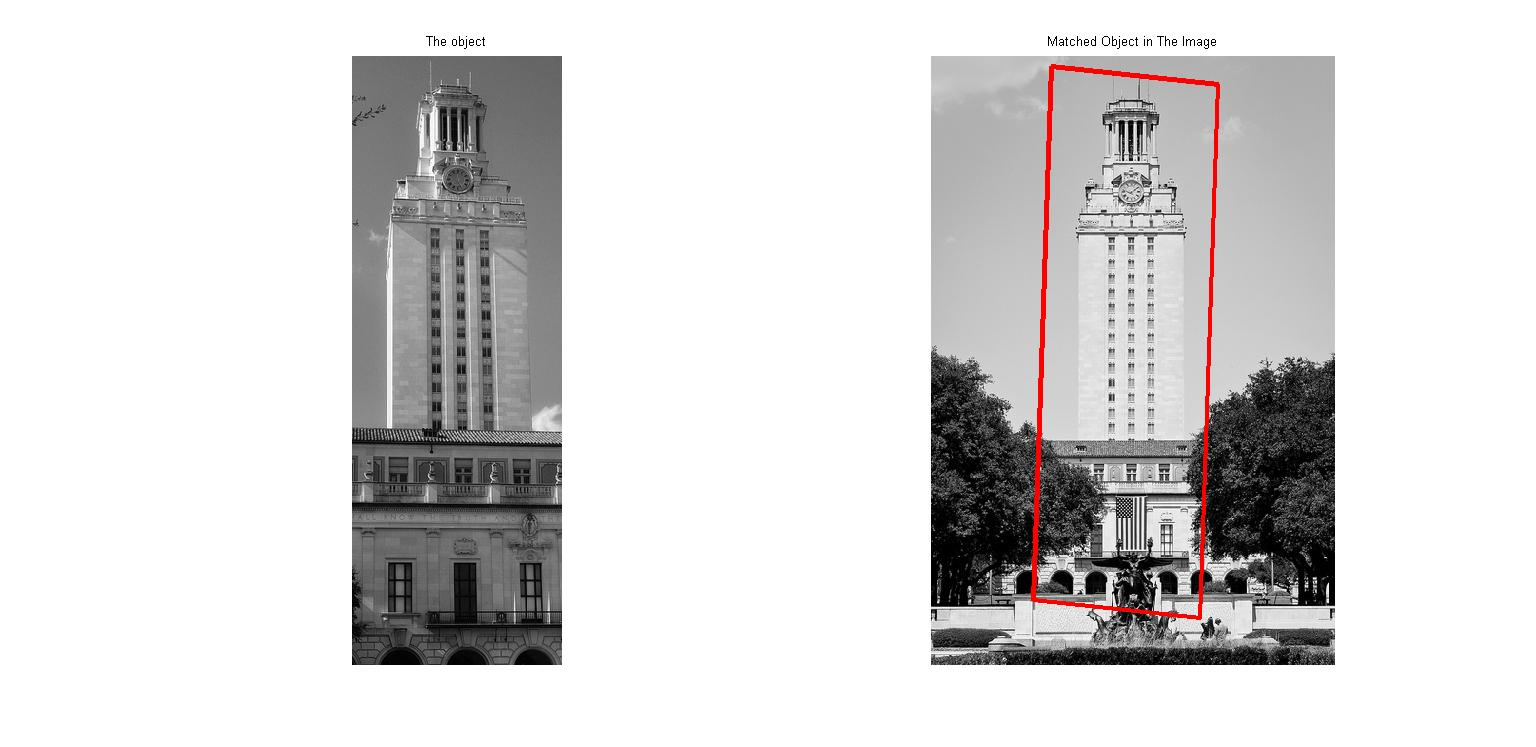
\includegraphics[width=\linewidth]{match_2.jpg}
  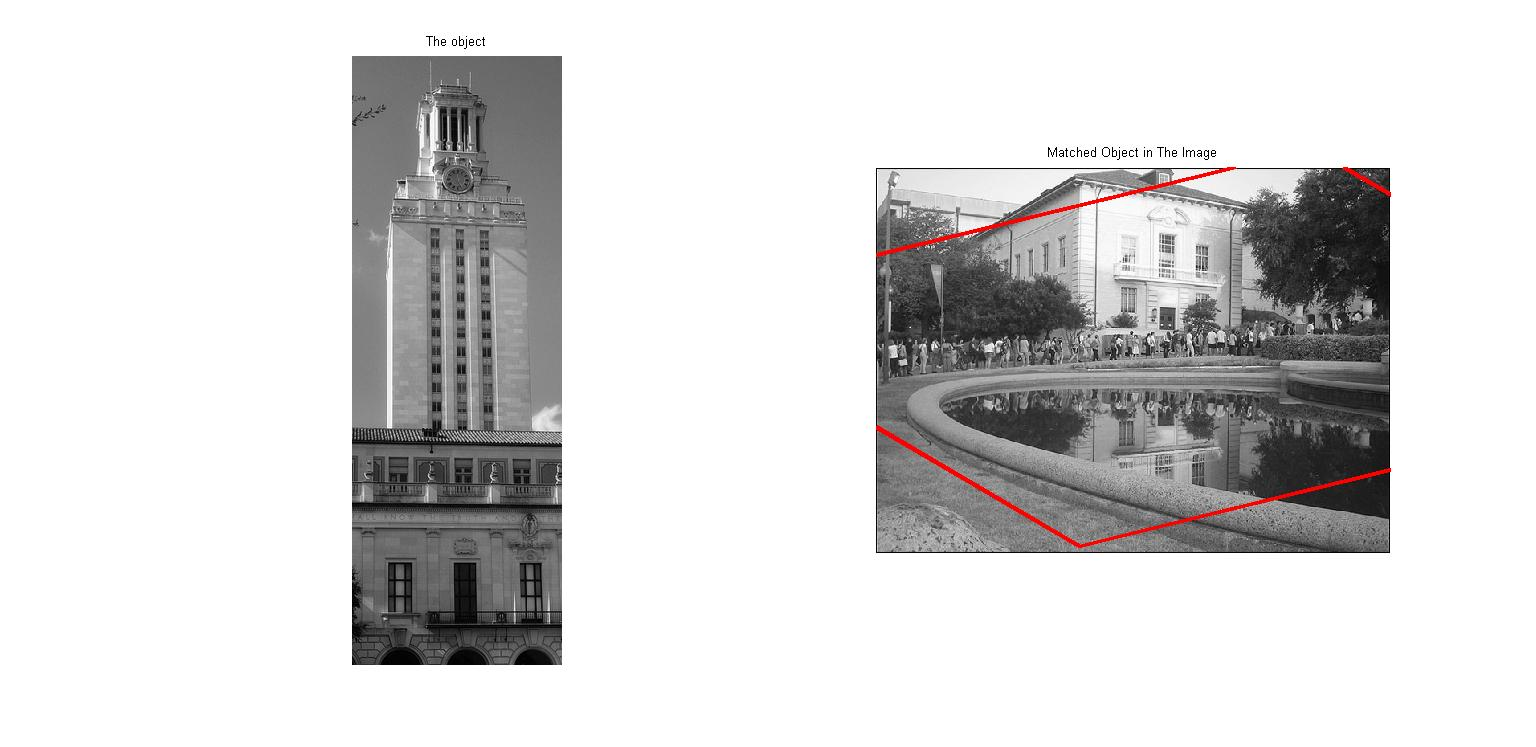
\includegraphics[width=\linewidth]{match_3.jpg}
\end{center}

\subsection{Extra Examples}
In this section, I will show two examples of matching, which is extra requirement.
\subsubsection{Stronger Variation}
This is a example of book in different rotation and illusion of the book on desk. 
\begin{center}
  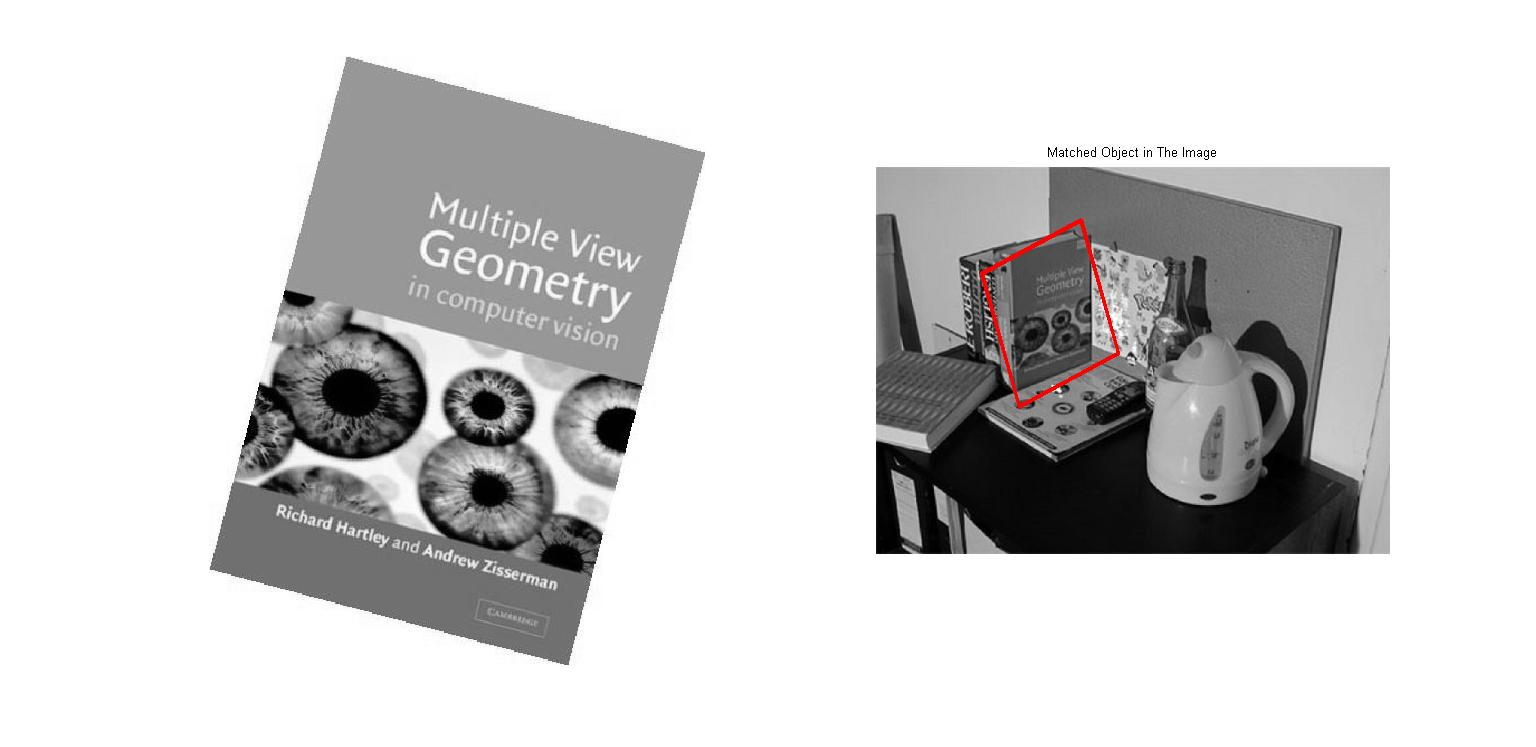
\includegraphics[width=\linewidth]{extra_1.jpg}
\end{center}

\end{spacing}

%\end{CJK*}
\end{document}
